\chapter{CLAMPING CIRCUIT}

\section*{AIM}
\paragraph{}To design and implement circuit for clamping waveforms
\section*{DESIGN AND CIRCUIT DIAGRAM}
\paragraph{}

Inorder to plot the transient response of clamping circuits use a SINE source whose amplitude, frequency, phase etc can be fixed during simulation. The SINE source is connected across a series connection of a diode and a capacitor and the output is taken across  the diode and the GND.The circuit for a clamper circuit is in Figure  \ref{clamper} .

\begin{figure}[h]
\centering
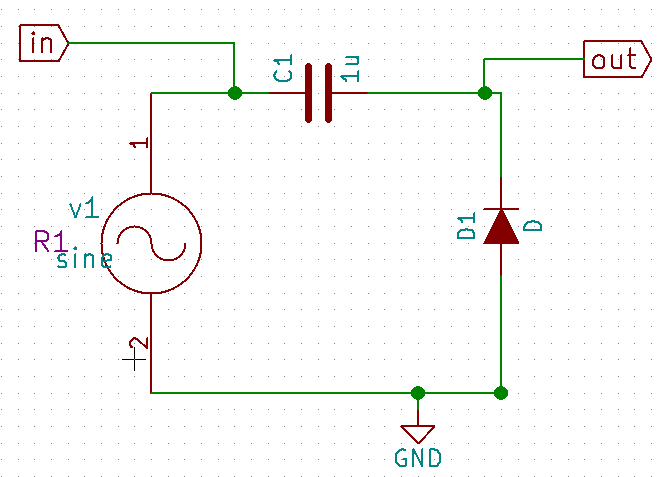
\includegraphics[width=0.8\textwidth]{clamper.png}
\caption{Schematic diagram for clamper circuit}
\label{clamper}
\end{figure}


\section*{PROCEDURE}

\paragraph{}The steps to plot the transint resonse of a clamper are explained below.. 
\subsection*{Launch eSim}

\paragraph{}
 Launching eSim will take you to the dialog box which asks for the default workspace. Browse the folders and set the wokspace location. It will finally end up in the eSim window.% shown in Figure \ref{LaunchWindow}.
%\begin{figure}[h]
%\centering
%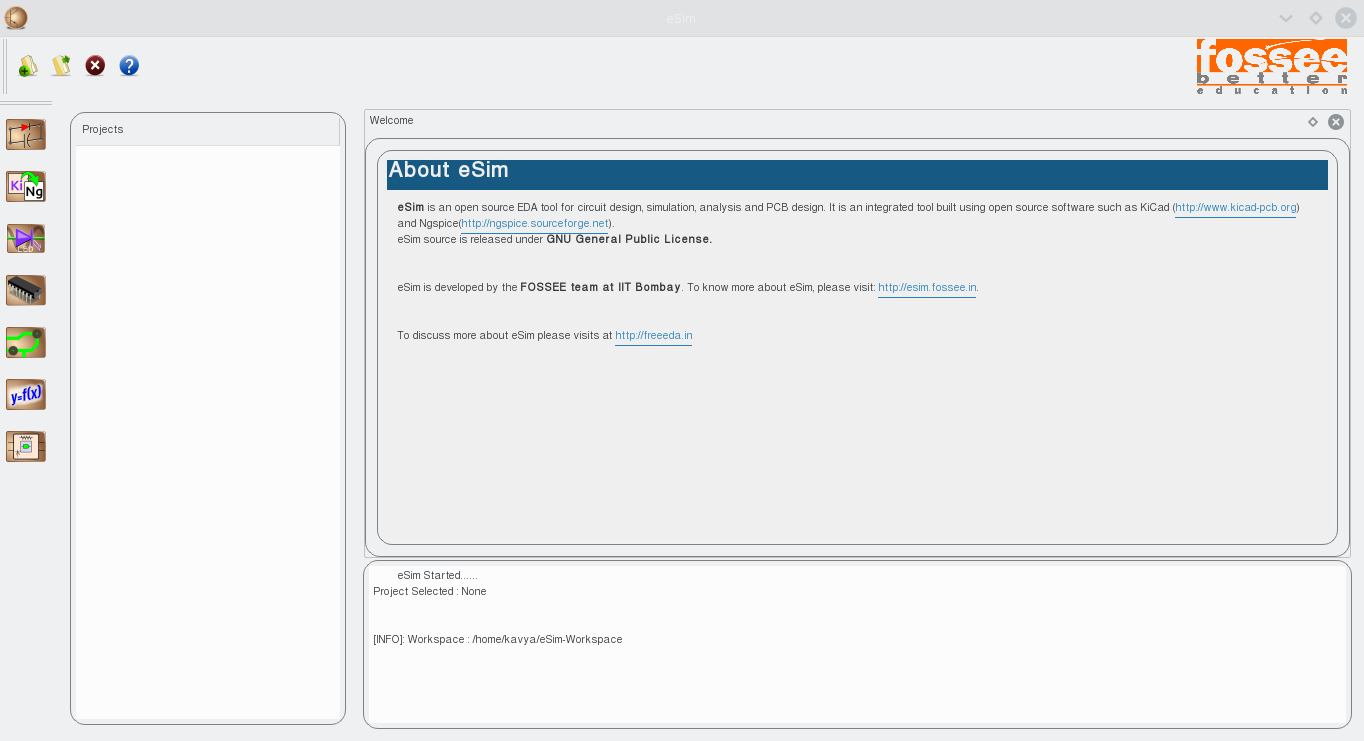
\includegraphics[width=0.8\textwidth]{LaunchWindow.png}
%\caption{Launching eSim will take you to this window}
%\label{LaunchWindow}
%\end{figure}

\subsection*{Create a New Project}

\paragraph{ } The new project is created by clicking the New icon on the
menubar. The name of the project is given in the pop up window as `clamper' for the circuit in Figure \ref{clamper}. Follow the steps explaied below to implement the circuit.
\subsection*{Create the Schematic}

\paragraph{}  To create the schematic, click the very first icon of the
left toolbar. This will open KiCad Eeschema.


To create a schematic in KiCad, we need to place the required components. After all the required components of the clipper circuit are placed, wiring is
done using the Place Wire option. The `Place Wire' and `Place Component' tools are available in the left toolbar. Scroll up and down for zooming in and out.


%\begin{figure}
%\begin{minipage}{.5\textwidth}
%  \centering
%  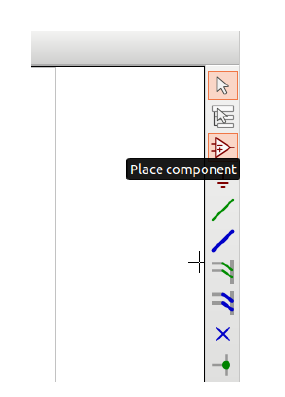
\includegraphics[width=\linewidth]{placecomponent.png}
%  \caption{Place component icon}
%  \label{placecomponent}
%\end{minipage}%
%\begin{minipage}{.5\textwidth}
%  \centering
%  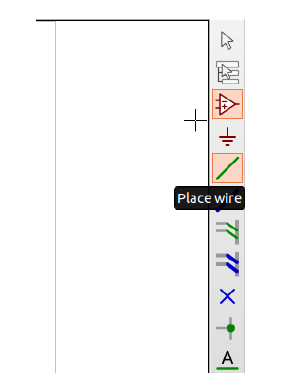
\includegraphics[width=\linewidth]{placewire.png}
%  \caption{Place wire icon}
%  \label{placewire}
%\end{minipage}
%\end{figure}


\paragraph{Placing the Components:} Normally all the components availbale in eSim can be chosen by left mouse click in the grid. The components are listed in different libraries. %See Figure \ref{librarylist}.

%\begin{figure}[h]
%\centering
%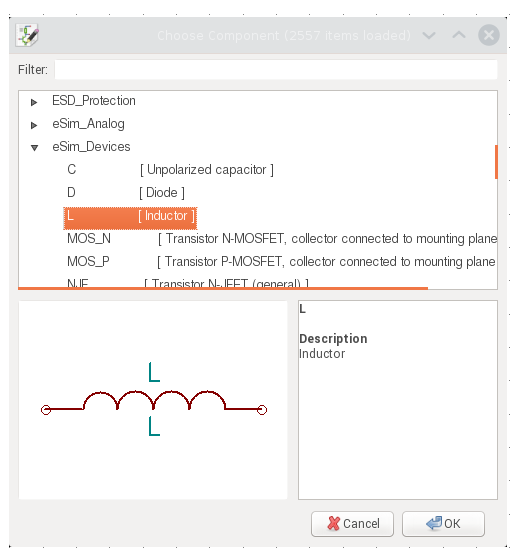
\includegraphics[width=0.5\textwidth, height=4cm]{librarylist.png}
%\caption{The Kicad Libraries of components}
%\label{librarylist}
%\end{figure}

\begin{itemize}
\item
Choose SINE source from eSim\_Sources
\item
Choose C from eSim\_Devices
\item
Choose D from eSim\_Devices
\item
Choose GND from power
\end{itemize}

Select the capacitor and edit its component value to 1u.% as shown in Figure \ref{editvalueRes}.

%\begin{figure}[h]
%\centering
%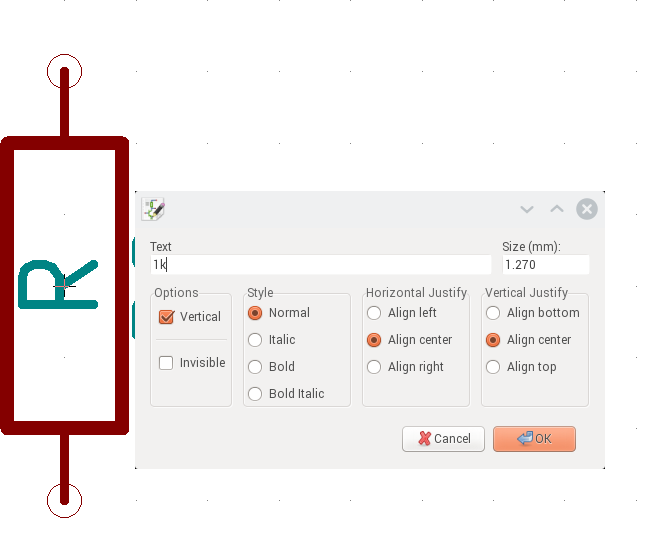
\includegraphics[width=0.5\textwidth, height=6cm]{editvalue.png}
%\caption{Editing the value field of component R}
%\label{editvalueRes}
%\end{figure}

Wire the components to get the circuit. A global label `in'  and `out' has been added to identify the node whose voltage will be later recorded and plotted. Global label is added from the right toolbar of Eeschema.

\paragraph{Annotating the circuit:} Once the schematic diagram is completed, annotate it so that the `question marks' associated with the components are converted to meaningful numbers automatically. Choose annotate button from the top toolbar and in the subsequenct dialogue boxes appearing click ok and finally close. See Figure \ref{annotationclamp}.

%\begin{figure}[h]
%\centering
%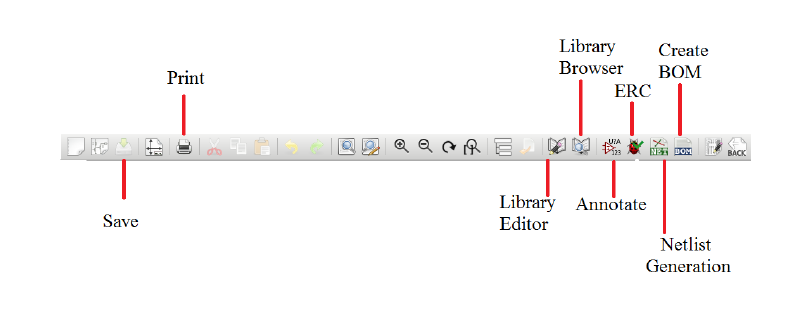
\includegraphics[width=\textwidth, height=4cm]{toptoolbar.png}
%\caption{Choose annotate from the toop tool bar}
%\label{toptoolbarclip}
%\end{figure}



Now we have the circuit diagram as shown in Figure \ref{clamper}.


\paragraph{Note:} If some libraries are found missing, you can add them from the `Preferences` menu by following the procedure: 

\begin{enumerate}
\item
Choose `Component Libraries' from Preferences menu.

\item
Click on the Add button on the top right side of the window.

\item
Choose the required libraries from `user/share/kicad/library' and click OK button

\end{enumerate}

\subsection*{Create Netlist}

\paragraph{}To simulate the circuit that has been created in the previous section, we need to generate
its netlist. Netlist is a list of components in the schematic along with their connection
information. To do so, click on the Generate netlist tool from the top toolbar. Click on
spice from the window that opens up. Check the option Default Format. Then click
on Generate. Save the netlist. This will be a .cir file. Do
not change the directory while saving. See Figure \ref{createnetlistclamp}.
 Now the netlist is ready to be simulated. 
\begin{figure}
\begin{minipage}{.5\textwidth}
  \centering
  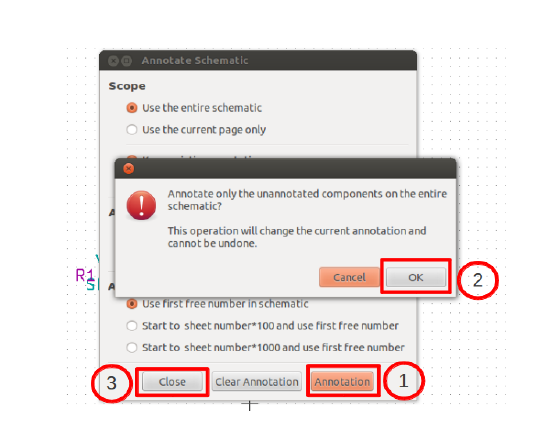
\includegraphics[width=\linewidth]{annotation.png}
  \caption{Annotation}
  \label{annotationclamp}
\end{minipage}%
\begin{minipage}{.5\textwidth}
  \centering
  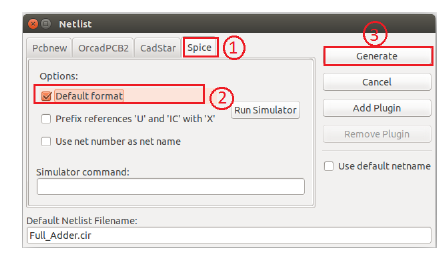
\includegraphics[width=\linewidth]{createnetlist.png}
  \caption{Netlist Generation}
  \label{createnetlistclamp}
\end{minipage}
\end{figure}

\subsection*{KiCad to Ngspice conversion}

\paragraph{} To convert KiCad netlist of clipper circuit to NgSpice
compatible netlist click on KiCad to Ngspice icon .  Now you can choose the type of analysis, source details, device models ngspice models and subcircuit models.


%\begin{figure}[h]
%\centering
%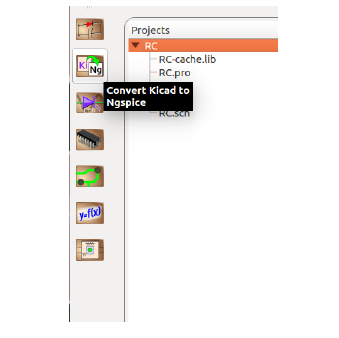
\includegraphics[width=0.5\textwidth, height=4cm]{kcd2spice.png}
%\caption{Choose Kicad to Ngspice tool}
%\label{kcd2spiceclip}
%\end{figure}
%

\paragraph{Analysis:}Choose analysis type as `Transient'.  Give the values of time variables as shown in Figure \ref{clampertransient}. Enter the time to be varied from `Start time=0 ms' to `Stop time=4ms' with a `Step time=0.01 ms'.

\begin{figure}[h]
\centering
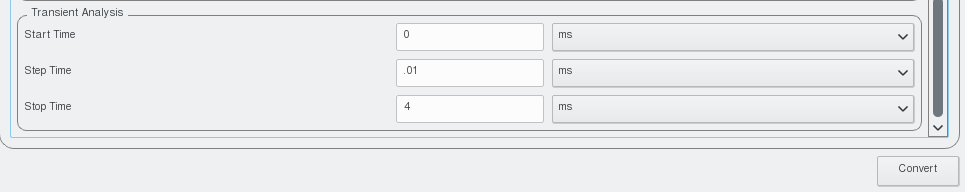
\includegraphics[width=\textwidth, height=4cm]{clampertransient.png}
\caption{Choose analysis type as `transient' and enter the values}
\label{clampertransient}
\end{figure}

\paragraph{Source Details:} Set the details of `sine' source as shown in Figure \ref{sinesource}.
\begin{itemize}
\item
Offset value(volts): 0
\item
Amplitude(volts): 4
\item
Frequency(Hz): 1k
\item
Delay time(Seconds): 0
\item
Damping factor(1/seconds):0

\end{itemize}
\begin{figure}[h]
\centering
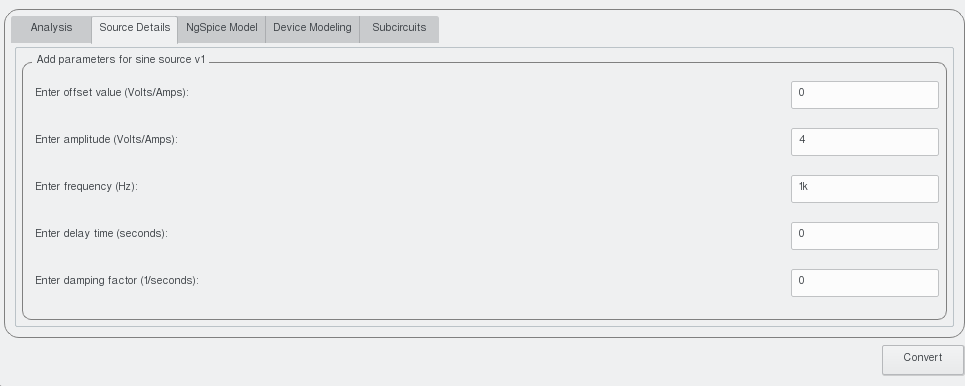
\includegraphics[width=\textwidth, height=4cm]{sinesourceclamper.png}
\caption{Enter the parameters of `Sine' source}
\label{sinesourceclamper}
\end{figure}


\paragraph{Ngspice Model:} No Ngspice model to be given.

\paragraph{Device Model:} Add the  diode model availablein the eSim library by browsing the folder, \texttt{/opt/eSim/src/deviceModelLibrary/Diode/D.lib}

\paragraph{Subcircuits:} No subcircuits to be given.

\noindent Once these details are provided click on convert button.  Now you are ready to see the simulation results.


\paragraph{}
\subsection*{Simulate} To run Ngspice simulation click the simulation icon in the left tool bar. It will open up two windows - ngspice plotting window and python plotting window. Inorder to plot the transient response of the clipper you can use either plotting types.

\paragraph{Python plotting:}This provides a graphical interface for plotting. We need to plot the value of voltage across the `SINE' source as well as the diode with respect to time. We have already labled these nodes as \texttt{in} and \texttt{out} respectively The nodes will be listed on the GUI. Choose  `in' and `out' and click on `plot' button. See Figure \ref{clamperpython}.

\begin{figure}[h]
\centering
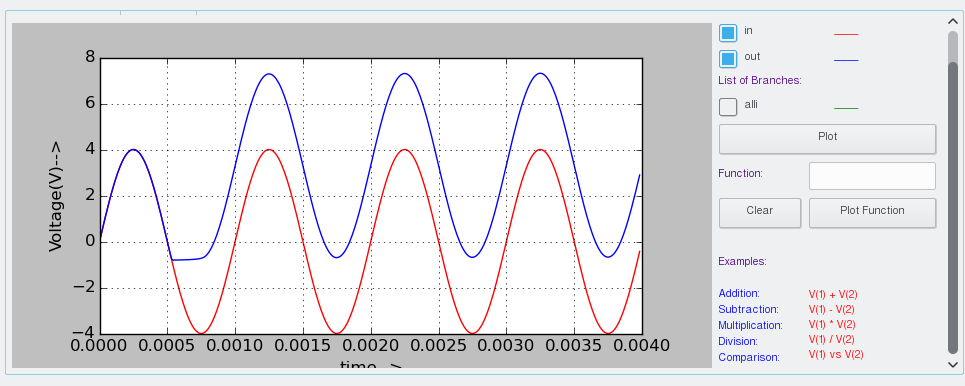
\includegraphics[width=12cm, height=8cm]{clamperpython.png}
\caption{The transient response of the clamper on python plotting window}
\label{clamperpython}
\end{figure}

\paragraph{Ngspice plotting:}. Time of simulation has already been set in the previous step. Use the commands in ngspice plotting window for obtaining the required plots.

\texttt{plot v(out), v(in) }

\paragraph{}

This would plot the transient response of input and output of the clamper. 


\section*{RESULT}
The circuit for plotting the transient analysis of clamper was implemented and simulated.


